%**************************************************************************
\section{Posters}\label{sec:posters}
%**************************************************************************

Participants were encouraged to bring posters to present
their recent research work.

%-- Hagen Paul Pfeifer
\subsection{Dynamic MultiPath Routing}

Safety critical communication platforms often deploy multiple heterogeneous
wireless link layer access technologies like ETSI TETRA, IEEE 802.11, IEEE
802.15.4, 3GPP LTE, satellite terminals or proprietary waveforms.  Depending
on the interface characteristics, vendor specific decisions and other aspects,
these often come shipped with suitable mobile ad-hoc routing protocols to form
networks in an autonomous manner - independently for each link type. 802.11
links typically deploy OLSR, BATMAN or 802.11s, whereas proprietary waveforms
often come with proprietary MANET protocols.  To bridge these access networks
at a logically higher level and provide an opaque operational network view, a
network routing protocol at the top is required. Exterior routing protocols
like BGP are limited in their use and features like automatic neighbor
detection or reduced message overhead are required. \ac{DMPR} tries to address
these shortcomings and provides exterior routing protocol features for
heterogeneous link layer environments even in low bandwidth environments.
Furthermore, \ac{DMPR} features policy based routing to route traffic through
different paths if required or advantageous.

%-- Michio Honda
\subsection{PASTE: A Networking Interface for NVMMs}

Emerging Non-Volatile Main Memories (NVMMs), also known as storage-class
memory and persistent memory  push the majority of end-to-end latency that
includes durable I/O to network stacks and their APIs.  This not only impairs
inherent performance of NVMMs that is one to two orders of magnitude faster
than traditional persistent medias like SSDs, but prevents systems from
adopting them to be reliable with relative ease. Michio Honda (NEC) presented
an investigation of this problem, designing an efficient network
stack~\cite{mhonda:hotnets:2016} and its APIs, and exploring new opportunities
in networking such as software switches and middleboxes in addition to
improving networked storage systems.

%-- Ermias Walelgne
\subsection{Measuring the Performance of Mobile Users}

In a mobile network, the mobile terminal (MT) continuously exchanges link
related metrics and signals to the nearby base station to measure the strength
and quality of the received signal. \ac{QoS} metrics are used for handover
decisions and cell reselection.  A handover can occur if there is a strong
radio signal in the neighboring cell while the serving cell’s radio signal is
getting diminished.  However, previous studies~\cite{ssonntag:wcnc:2013} show
that it is not always the value of signal strength that matters to have a good
throughput performance.  Therefore, knowing the possible achievable throughput
value before making a handover is equally important along with link-related
\ac{QoS} metrics. Ermias Walelgne (Aalto University) proposes a solution to
estimate the throughput value of post-handover using the metrics collected
from the current serving base station. The result of this throughput
prediction can be combined with other link QoS metrics such as RSSI and RSPQ
values for better handover decision.


%-- Roberto Morabito
\subsection{Lightweight Virtualization for Smart Cars}

Modern vehicles are equipped with several interconnected sensors on board for
monitoring and diagnosis purposes; their availability is a main driver for the
development of novel applications in the smart vehicle domain. Roberto
Morabito~\cite{rmorabito:im:2017} presented a Docker container-based platform
as solution for implementing customized smart car applications. Through a
proof-of-concept prototype—developed on a Raspberry Pi3 board—we show that a
container-based virtualization approach is not only viable but also effective
and flexible in the management of several parallel processes running on
On-Board Unit. More specifically, the platform can take priority-based
decisions by handling multiple inputs, e.g., data from the CANbus based on the
OBD II codes, video from the on-board webcam, and so on. Results are promising
for the development of future in-vehicle virtualized platforms.

%-- Ljubica Pajević Kärkkäinen
\subsection{Data-driven Mobility Modeling}

Ljubica Pajević Kärkkäinen (TU Munich) presents an analysis of a large trace
of user associations in a university wireless network, which includes around
one thousand access points on five campus sites. The trace was obtained from
authentication logs of the RADIUS server collected over 16 months.  User
access patterns, specifically the arrival processes of users to wireless
access points, visiting time duration, as well as the user arrival patterns to
the buildings in the campus are studied. She observed that that a large
fraction of the network -- around half of all access points -- exhibit Poisson
arrival process, which is advantageous for modeling and prediction of network
occupancy. By analyzing duration of associations with access points, she shows
that the visiting time distributions can be modeled by two-stage
hyper-exponential distributions.  While network associations in campus
wireless networks have been extensively studied in the literature, this study
reveals changing access patterns, which seem to be characteristic for networks
of predominantly mobile users.

%-- Michael Haus
\subsection{iConfig - What I See is What I Configure}

Michael Haus (TU Munich) presented iConfig to manage \ac{IoT} devices in smart
cities. The management of \ac{IoT} devices in urban areas is becoming
important due to that the majority of the people living in cities and the
number of deployed \ac{IoT} devices are increasing. Therefore, iConfig
addresses three major issues in current \ac{IoT} management: registration,
configuration, and device maintenance. To achieve the goals of iConfig, the
presented system relies on programmable edge modules, which can run on
smartphones, wearables, and smart boards to configure physically proximate
\ac{IoT} devices.


%-- Teemu Kärkkäinen
\subsection{Opportunistic Content Dissemination}

Many of the existing opportunistic networking systems have been designed
assuming a small number links per node and have trouble scaling to large
numbers of potential concurrent communication partners. In the real world we
often find wireless local area networks with large numbers of connected users
– in particular in open Wi-Fi networks provided by cities, airports,
conferences and other venues. In this talk, Teemu Kärkkäinen (TU Munich)
presented a 50 client opportunistic network in a single Wi-Fi access point and
use it to uncover scaling problems and to suggest mechanisms to improve the
performance of single segment dissemination. Further, we present an algorithm
for breaking down a single dense segment dissemination problem into multiple
smaller but identical problems by exploiting resource (e.g., Wi-Fi channel)
diversity, and validate our approach via simulations and testbed experiments.
The ability to scale to high density network segments creates new, realistic
use cases for opportunistic networking applications.


%-- Daniel Herzog
\subsection{A Group Recommender System for Trips}

\ac{RSs} in tourism often recommend single \ac{POIs} such as restaurants or
museums. However, tourists visiting a destination are usually looking for a
tourist trip composed of multiple \ac{POIs} along a practical route. Daniel
Herzog (TU Munich) presented a \ac{RS}~\cite{dherzog:it:2017} recommending
tourist trips to a group of users.  This is a particularly complex problem as
the \ac{RS} has to aggregate the travel preferences of all group members
before generating recommendations. Furthermore, he wants to research on how
different devices and user interfaces can support groups in providing feedback
on recommendations and finding a consensus.

%-- Lars Wischhof
\subsection{Data Dissemination in Vehicular Networks}

Lars Wischhof (Hochschule Müncher) presented an architecture and preliminary
results of an on-going research project at the research group where
communication schemes combining cellular communication with
direct-communication (such as \ac{D2D} modes of the latest LTE-A releases or
LTE-V) are combined for applications in intelligent mobility. The basic
assumption is that future vehicles will most-likely have multiple
communication technologies and modes available. Therefore, a context-aware
selection of the communication mode is advocated. A suitable architecture is
outlined. First simulation results for the example of a DENM-based application
indicate that a context-aware selection can outperform a static assignment.


%-- Severin Kacianka
\subsection{Accountability for Cyber-Physical Systems}

Severin Kacianka (TU Munich) seeks to capture the essential features of an
accountable (computer-)system.  Logs are, for example, a common way to create
evidence and establish  "truth" in computer systems. Another facet are
mechanisms to process those logs and techniques to formulate the questions of
compliance with laws as queries against those logs.  However, there are
currently no "blue prints" on how to make a system "accountable". We wish to
develop a comprehensive framework that makes it possible to explicate the
accountability features of a system, reason about their effectiveness, compare
it to other solutions and offer options to exchange one specific component for
another.


%-- Edwin Cordeiro
\subsection{Real-time TE in the Internet}

Edwin Cordeiro (TU Munich) aims to create a network solution capable of
detecting and avoiding congestions in the Internet. The avoidance is done
automatically by a central controller adapting running network protocols and
network routes to avoid congestion.  Such objectives are divided in two parts.
The first one is the creation of a method capable of detecting congestion in
the Internet in real-time without probes at destinations. The second is the
implementation of \ac{SDN} ideas in the routing system using the \ac{I2RS}
protocol, that is being specified by \ac{IETF}.

%-- Vittorio Cozzolino
\subsection{Fine-Grained Edge Offloading for IoT}

Vittorio Cozzolino (TU Munich) makes the case for \ac{IoT} edge offloading,
which strives to exploit the resources on edge computing devices by offloading
fine-grained computation tasks from the cloud closer to the users and data
generators (i.e., IoT devices). The key motive is to enhance performance,
security and privacy for IoT services. The proposal bridges the gap between
cloud computing and IoT by applying a divide and conquer approach over the
multi-level (cloud, edge and IoT) information pipeline.  To validate the
design of IoT edge offloading, a unikernel-based prototype is developed and
evaluated the system under various hardware and network conditions.

%-- Stefan Neumeier
\subsection{CARISSMA}

\ac{CARISSMA} is a new center for vehicle safety. Its focus is on passive as
well as active vehicle safety research. The main goal is to develop a global
safety system to support 'Vision Zero', achieving the ultimate goal of zero
traffic deaths. Therefore, all relevant disciplines are combined in one
building. Nine professors alongside 47 staff members pursue are working in, e.
g. an indoor driving area and full-vehicle crash test facility, a drop tower,
a HiL-lab, a full-vehicle test bench, a lab for safe energy storage, a
car2x-laboratory, a simulation lab and an open-air ground for performing
full-vehicle tests.

\subsection{Car2X Lab}

Research on Car2X communication, the wireless communication between vehicles
and other road participants, is gaining a major part of \ac{CARISSMA}. The
Car2X research facilities feature a powerful simulation computer, which helps
to leverage our Open Source in-house Car2X simulation tools “Artery” and
“Vanetza”. These tools will also be integrated in our Car2X experimental
vehicle, blending virtual simulation and real test drives for semi-virtualized
testing. In addition to this, the research is focusing on HIL-testing of Car2X
equipment. Further research topics are Teleoperated Driving and the use of
Mobile Edge Computing for vehicular applications.

%-- Nemanja Deric
%\subsection{SENDATE - Secure Networking for a Data Center Cloud in Europe}
\subsection{SENDATE}

The goal of the SENDATE sub-project PLANETS is to provide cutting edge technical
and scientific solutions for ProgrammabLe Architecture for distributed NETwork
functions and Security. As TUM's Lehrstuhl für Kommunikationsnetze (LKN) is
one of the main contributors of the SENDATE PLANETS, this poster aims to
present an overview of only some of the research directions of LKN. The most
related work could be classified as i) Network virtualization evaluation,
hypervisor control plane migration protocol (i.e. DITRA) and HyperFlex
virtualization platform, ii) Resilient network design and planning \& techno
economic analysis and iii) Hypervisor placement, performance evaluation and
mapping and synthetic IP graph generation.

\begin{figure*}[t!]
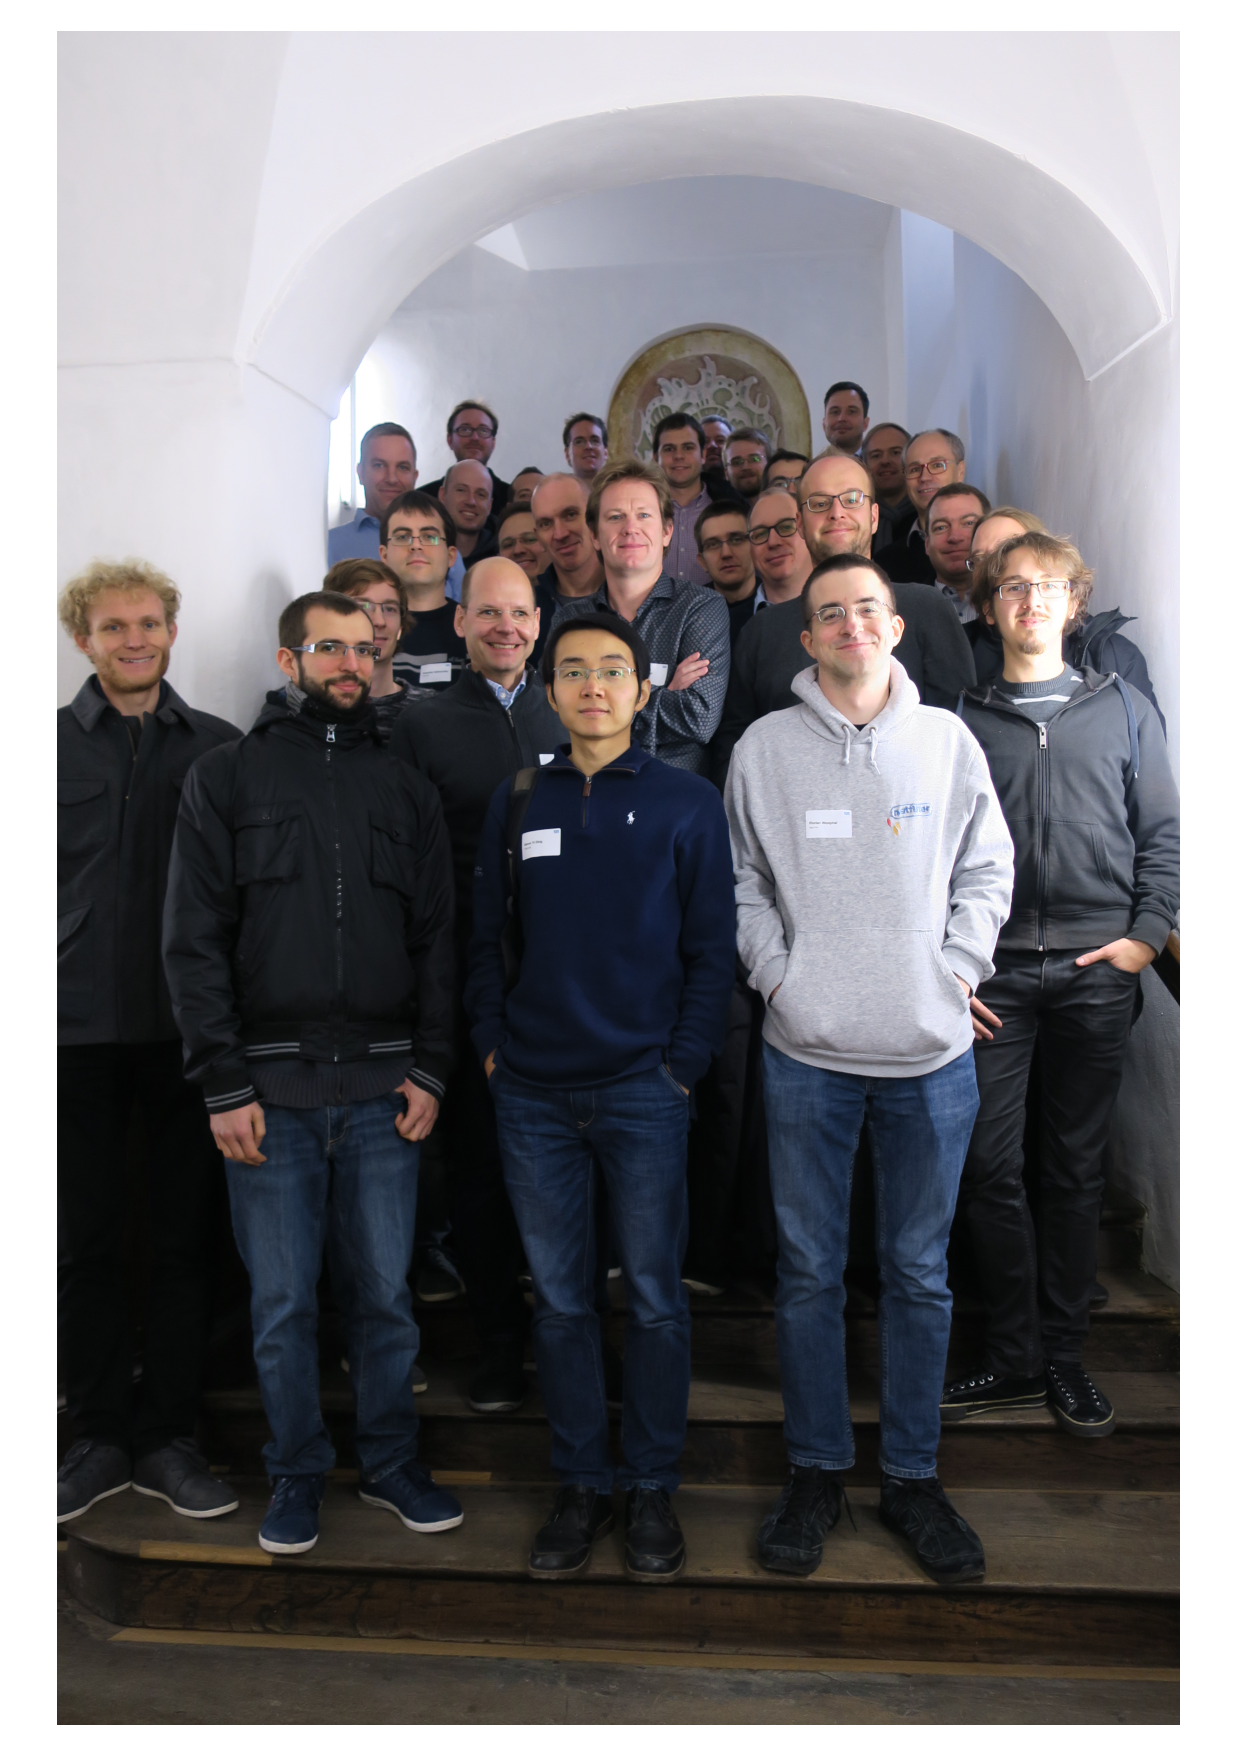
\includegraphics[width=\linewidth]{figures/group-photo}
\end{figure*}

%-- Alberto Martínez:
%\subsection{FlexNets - Quantifying Flexibility in Communication Networks}
\subsection{Quantifying Flexibility in Networks}

Communication networks need to face fast and frequent changes, since the
request of resources from users is increasingly dynamic. Several new
technologies have arisen to deal with this requirement, such as Software
Defined Networking (SDN), Network Virtualization (NV) and Network Function
Virtualization (NFV). These technologies claim to enhance the flexibility of
the network, i.e., the ability of the network to adapt to changes. However, a
formal definition of flexibility has not been settled, thus it is difficult to
measure and compare the performance of these technologies. Alberto Martinez
(TU Munich) proposed an initial definition of flexibility and we illustrate it
with an use case: the dynamic placement of the controller in a SDN-enabled
network.

%— Quirin Scheitle
%\subsection{Internet Architecture and its Security Implications}
\subsection{Internet Architecture and Security}

Quirin Scheitle (TU Munich) presented research directions in both Internet
Architecture and Security questions.  Examples for this are Geolocation of
Routers using Ripe Atlas~\cite{glra}, mapping the communication flows and
backend infrastructures of Mobiles Messaging Services such as WhatsApp or
WeChat~\cite{mms}, and about creation and operation of an IPv6
hitlist~\cite{ipv6hitlist}.

